% !TeX root = ../Book1.tex
\begin{figure}[htbp]
	\centering
	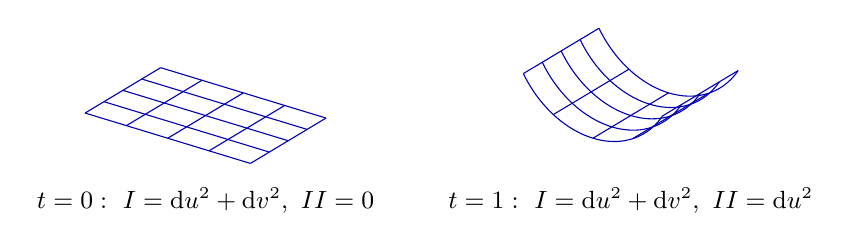
\begin{tikzpicture}[x={(1.05cm,-0.32cm)},y={(0.6cm,0.36cm)},z={(0cm,1.2cm)},font=\small]
		\begin{scope}[xshift=-2.8cm]
			\foreach \a in {-1,-0.5,0,0.5,1}{\draw[blue!70!black] (\a,-0.8,0)--(\a,0.8,0);}
			\foreach \b in {-0.8,-0.4,0,0.4,0.8}{\draw[blue!70!black] (-1,\b,0)--(1,\b,0);}
			\node at (0,0,-0.9) {\(t=0:\ I=\mathrm{d}u^2+\mathrm{d}v^2,\ II=0\)};
		\end{scope}
		\begin{scope}[xshift=2.6cm]
			\foreach \a in {-1,-0.5,0,0.5,1}{\draw[blue!70!black] ({sin(deg(\a))},-0.8,{1-cos(deg(\a))})--({sin(deg(\a))},0.8,{1-cos(deg(\a))});}
			\foreach \b in {-0.8,-0.4,0,0.4,0.8}{\draw[blue!70!black,domain=-1:1,samples=41,variable=\a] plot ({sin(deg(\a))},\b,{1-cos(deg(\a))});}
			\node at (0,0,-0.9) {\(t=1:\ I=\mathrm{d}u^2+\mathrm{d}v^2,\ II=\mathrm{d}u^2\)};
		\end{scope}
	\end{tikzpicture}
	\caption[平面卷成圆柱片]{同一参数网格的等距形变。两图的第一基本形式相同；弯曲后沿 \(u\) 方向的法向随位置改变，第二基本形式随之改变。图中采用例中的法向约定。}
	\label{g1:fig:plane-cylinder-bending}
\end{figure}
